% ---------------------- Smart Recycler Technical Report --------------------- %
% Authors:
%   Ayrton Albuquerque
%   Ian D. A. Queros
%   Miguel Chagas
% ------------------------------------ END ----------------------------------- %

% ---------------------------------------------------------------------------- %
%                                   Packages                                   %
% ---------------------------------------------------------------------------- %
\documentclass[a4paper,11pt]{article}
\usepackage[english]{babel}
\usepackage[utf8]{inputenc}
\usepackage[T1]{fontenc}
\usepackage{fancyhdr}
\usepackage{fancybox}
\usepackage{easylist}
\usepackage{paralist}
\usepackage{pbox}
\usepackage[hyphens]{url}
\usepackage{multirow}
\usepackage{array, hhline}
\usepackage{fourier}
\usepackage{ifsym}
\usepackage{graphicx}
\usepackage{float}
\usepackage{pdfpages}
\usepackage[pdftex]{hyperref}
\usepackage{color}

\pagestyle{fancy}
\definecolor{corlinkprint}{rgb}{0, 0, 0}
\hypersetup{
  colorlinks,
  citecolor   = corlinkprint,
  filecolor   = corlinkprint,
  linkcolor   = corlinkprint,
  urlcolor    = corlinkprint}

% ---------------------------------------------------------------------------- %
%                                    Header                                    %
% ---------------------------------------------------------------------------- %
\fancyhead[L]{\small{Technical Report: Smart Recycler}}
\fancyhead[R]{\small\thepage} 
\fancyfoot{}
\renewcommand\headrulewidth{0.4pt}

% ---------------------------------------------------------------------------- %
%                                     Title                                    %
% ---------------------------------------------------------------------------- %
\title{
Technical Report\\
\textbf{Smart Recycler}}

% ---------------------------------------------------------------------------- %
%                                    Authors                                   %
% ---------------------------------------------------------------------------- %
\author{
Ayrton Albuquerque \footnotesize{-- ayrtonsilva@alunos.utfpr.edu.br}\\
Ian D. A. Queros \footnotesize{-- ianqueros.1996@alunos.utfpr.edu.br}\\
Miguel Chagas \footnotesize{-- migueln@alunos.utfpr.edu.br}\\
}

% ---------------------------------------------------------------------------- %
%                                     Date                                     %
% ---------------------------------------------------------------------------- %
\date{June, 2022}

% ---------------------------------------------------------------------------- %
%                                   Document                                   %
% ---------------------------------------------------------------------------- %
\begin{document}

% ----------------------------- First Page Header ---------------------------- %
\thisfancyput(35mm,-10mm){
  \begin{tabular}{c}
    Federal University of Technology - Paraná - Brasil -- \small{UTFPR} \\
    Academic Department of Electronics -- \small{DAELN}                 \\
    Academic Department of Informatics -- \small{DAINF}                 \\
    Computer Engineering                                                \\
    Integration Workshop 3 (EEX23) -- S71 -- 2022/1                     \\
    \\
    \hline
  \end{tabular}}

% --------------------------------- Maketitle -------------------------------- %
\maketitle

% --------------------------------- Abstract --------------------------------- %
\begin{abstract}
  \noindent In a society that produces more waste with each passing year, the separation of what is recyclable and what is not can become a problem. When discarding materials, people tend to not pay to much attention if something is recyclable or not and, when not properly segregated, those materials end up if field dumps never to be seen or reused again. Our project comes as a possible solution to this problem and to help defining a clear scope we choose the university environment. The system consists of an automated trash bin for some types of recyclable waste, such as some specific kinds of papers, plastics, and metals. The separation is done using image classification, where a picture of the discarded waste is taken and analyzed by a neural network, and using a set of motors attached to flaps the item is moved to a specific container. As incentive for recycling we are also rewarding the users with symbolical credits that could be used in different ways. The present document details the development of the project.
\end{abstract}

% ---------------------------------------------------------------------------- %
%                                     Body                                     %
% ---------------------------------------------------------------------------- %
\section{Introduction}
\label{sec:intro}
\noindent

Waste management has always been a challenge in modern society due to population growth and technological advancements enabling significant incre\-ases in waste production. In Brazil 79.1 million tons of solid waste are generated each year \cite{Senado} of which 92\% is collected, but only 59.5\% of those reach a proper destination \cite{Senado}. When talking about recycling the picture is even more grim, only 2.1\% of all the waste collected is recycled \cite{Poder360} and most of this process is done through manual labor.

In day to day life people segregate waste in trash bins that are usually divided in recyclable and organic types, or in some cases the recyclables are divided in four categories and even then not much attention is put into throwing the waste in the correct bin. This makes a second separation process necessary because every material have its own recycle process.

To try solving this problem the Smart Recycler was conceptualized, a system that utilizes a image recognition network integrated to a embedded system that controls a sorting mechanisms, allowing waste to be thrown at it and automatically segregating to a proper container. The system also provides to the user an incentive for recycling through a symbolical credit compensation after scanning a qr code generated and displayed  by the system itself.

\subsection{Project Overview}
\label{subsec:overview}

\begin{figure}[H]
  \centering
  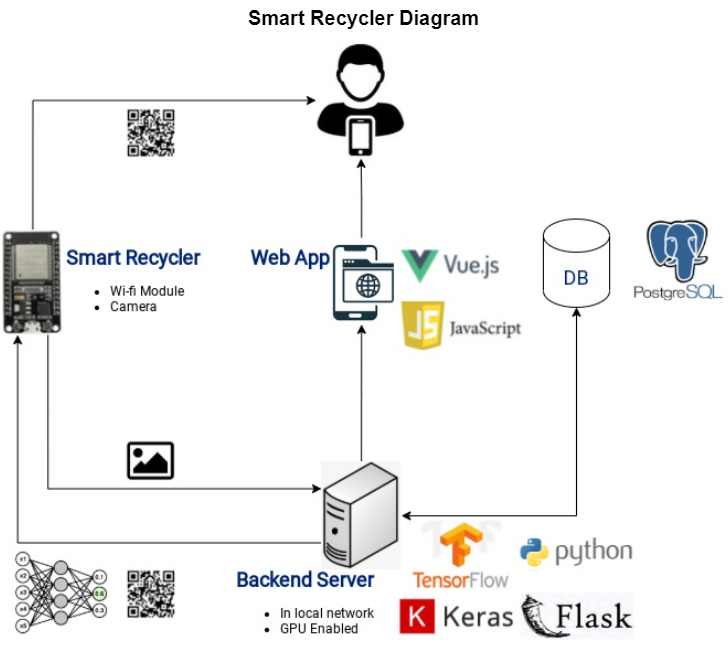
\includegraphics[width=10cm]{Figures/Smart Recycler Diagram.png}
  \caption{\small{Block diagram of the system}}
  \label{fig:blockDiagram}
\end{figure}

The project revolves around two main systems, the embedded system consisting of two micro-controllers and the inference system responsible for classifying the waste images. The first micro-controller used is an ESP32-Cam, an Espressif micro-controller with an embedded 2 megapixels camera responsible for capturing the image of the waste item inside the Smart Recycler and bridging the communication between the back end system and the Arduino Mega, the second micro-controller responsible for controlling all the peripherals in the system.

The image classification takes place as soon as some item is thrown into the Smart Recycler. To detect this, an infrared sensor was used and after a brief period an image of the item inside is taken and sent to a back end system that classifies it, returning a JSON containing the item classification and a redeem code that will later be used to generate a \textit{QR Code}.

When the user scans the \textit{QR Code} he/she will be rewarded with a symbolical credit amount that is stored in a digital wallet. This wallet is part of a Web Application that was developed to help the user maintain its credits and visualize information about the waste recycled. The application also allows credit transactions between users.

An item can be classified as one of six classes defined in the project and can be disposed in one of the four containers, those being \textit{soda cans} disposed in the metal container, \textit{juice boxes} and \textit{crumpled paper} disposed in the paper container, \textit{plastic bottle}, \textit{plastic cup}, and \textit{chip bags} disposed in the plastic container and finally the fourth container is destined to \textit{others}.

Once an item is classified the recycle process begin by moving a set of three motors divided in two levels in coordination. The first level motor rotates to either left or right and depending on the classification, the second level motor will rotate to front or back. All the information generated during the recycle process is stored in a database and statistic about it can be seen in the web application.

\section{Project Specifications}
\label{sec:specification}
\noindent

The following subsections describe the requirements, components and tools used in the project development.

\subsection{Requirements}
\label{subsec:requirement}

The project requirements were divided in six areas of development based on the relationship between each technology used. The following tables present the requirements of each part of the project as they were implemented, starting with the mechanical requirements, followed by hardware, embedded, web application, back end and finally inference requirements.

% Mechanical System Requirements
\begin{table}[H]
  \small
  \caption{\small{Mechanical functional requirements}}
  \begin{center}
    \begin{tabular}{|c|p{95mm}|}
      \hline
      Requirement & Description                                                                    \\ \hline
      MS-FR01     & The Mechanical Structure must use flaps to direct the waste to its container   \\ \hline
      MS-FR02     & The Mechanical Structure must allow the emptying of waste containers           \\ \hline
      MS-FR03     & The Mechanical Structure must segregate the waste from the hardware components \\ \hline
      MS-FR04     & The Mechanical Structure must protect the hardware from fluids                 \\ \hline
    \end{tabular}
  \end{center}
  \label{tab:mechanical0}
\end{table}

\begin{table}[H]
  \caption{\small{Mechanical non-functional requirements}}
  \begin{center}
    \begin{tabular}{|c|p{95mm}|}
      \hline
      Requirement & Description                                                                                                             \\ \hline
      MS-NFR01    & The Mechanical Structure must have one container for each type of waste                                                 \\ \hline
      MS-NFR02    & The waste containers must have a 25x25 cm base and 60 cm height and the Smart recycler must be at most 150 cm of height \\ \hline
      MS-NFR03    & The Mechanical Structure must have a gate                                                                               \\ \hline
      MS-NFR04    & The Smart Recycler must have a detection chamber above its waste containers                                             \\ \hline
      MS-NFR05    & The mechanical structure must have cases for all the electronic devices for MS-FR04                                     \\ \hline
    \end{tabular}
  \end{center}
  \label{tab:mechanical1}
\end{table}

% Hardware System Requirements
\begin{table}[H]
  \caption{\small{Hardware functional requirements}}
  \begin{center}
    \begin{tabular}{|c|p{95mm}|}
      \hline
      Requirement & Description                                                                         \\ \hline
      HS-FR01     & The Hardware system must establish a Wi-Fi connection with the Backend              \\ \hline
      HS-FR02     & The Hardware system must control the flaps of the Mechanical Structure              \\ \hline
      HS-FR03     & The Hardware system must take pictures for material classification                  \\ \hline
      HS-FR04     & The Hardware system must detect the entrance of garbage in the Mechanical Structure \\ \hline
      HS-FR05     & The Hardware system must properly illuminate the detection chamber                  \\ \hline
      HS-FR06     & The Hardware system must display messages and QR Codes for the user                 \\ \hline
      HS-FR07     & The Hardware system must indicate when a container is nearing its capacity          \\ \hline
      HS-FR08     & The Hardware system will only process one type of garbage per time                  \\ \hline
    \end{tabular}
  \end{center}
  \label{tab:hardware0}
\end{table}

\begin{table}[H]
  \caption{\small{Hardware non-functional requirements}}
  \begin{center}
    \begin{tabular}{|c|p{95mm}|}
      \hline
      Requirement & Description                                                             \\ \hline
      HS-NFR01    & The Hardware system must have one WIFI module for HS-FR01               \\ \hline
      HS-NFR02    & The Hardware system must have a power supply                            \\ \hline
      HS-NFR03    & The Hardware system must have three servo motors for HS-FR02            \\ \hline
      HS-NFR04    & The Hardware system must have one camera for HS-FR03                    \\ \hline
      HS-NFR05    & The Hardware system must have an ultrasonic sensor for HS-FR04          \\ \hline
      HS-NFR06    & The Hardware system must have a led tape for HS-FR05                    \\ \hline
      HS-NFR07    & The Hardware system must have one OLED Display for HS-FR06              \\ \hline
      HS-NFR08    & The Hardware system must have four LEDs for HS-FR07                     \\ \hline
      HS-NFR09    & The whole process of garbage disposal must take a maximum of 15 seconds \\ \hline
    \end{tabular}
  \end{center}
  \label{tab:hardware1}
\end{table}

% Embedded System Requirements
\begin{table}[H]
  \small
  \caption{\small{Embedded functional requirements}}
  \begin{center}
    \begin{tabular}{|c|p{95mm}|}
      \hline
      Requirement & Description                                                                            \\ \hline
      ES-FR01     & The micro-controller must read the sensors signals in the Hardware system              \\ \hline
      ES-FR02     & The micro-controller must send signals to control the actuators in the Hardware system \\ \hline
      ES-FR03     & The micro-controller must detect when an object is thrown into the Smart Recycler      \\ \hline
      ES-FR04     & The micro-controller must control the flow of garbage to its correct container         \\ \hline
      ES-FR05     & The micro-controller must send the image to the Backend system                         \\ \hline
      ES-FR06     & The micro-controller must present the received QR Code in a screen for the user        \\ \hline
    \end{tabular}
  \end{center}
  \label{tab:embedded0}
\end{table}

\begin{table}[H]
  \small
  \caption{\small{Embedded non-functional requirements}}
  \begin{center}
    \begin{tabular}{|c|p{95mm}|}
      \hline
      Requirement & Description                                                                                                \\ \hline
      ES-NFR01    & The embedded system must have a micro-controller                                                           \\ \hline
      ES-NFR02    & The picture of the thrown object must be taken 5 seconds after the gate’s infrared sensors gets obstructed \\ \hline
      ES-NFR03    & The micro-controller must have Wi-Fi connection to use image processing and QR Code                        \\ \hline
      ES-NFR04    & The software for the embedded system must be written in C                                                  \\ \hline
      ES-NFR05    & When a container is full, its content must be classified as “other”                                        \\ \hline
    \end{tabular}
  \end{center}
  \label{tab:embedded1}
\end{table}

% Web App System Requirements
\begin{table}[H]
  \caption{\small{Web Application functional requirements}}
  \begin{center}
    \begin{tabular}{|c|p{95mm}|}
      \hline
      Requirement & Description                                                                \\ \hline
      F-FR01      & The Web App must allow users to sign in and sign up in the system          \\ \hline
      F-FR02      & The Web App must allow users to visualize their credit balance             \\ \hline
      F-FR03      & The Web App must allow users to send credits to other user                 \\ \hline
      F-FR04      & The Web App must allow users to visualize statistics about waste collected \\ \hline
      F-FR05      & The Web App must allow users to scan QR Codes using their phone camera     \\ \hline
      F-FR06      & The Web App must allow users to report a problem about the Smart Recycler  \\ \hline
    \end{tabular}
  \end{center}
  \label{tab:app0}
\end{table}

\begin{table}[H]
  \caption{\small{Web Application non-functional requirements}}
  \begin{center}
    \begin{tabular}{|c|p{95mm}|}
      \hline
      Requirement & Description                                                                                                  \\ \hline
      F-NFR01     & The Web App sign up form will contain the following text fields: e-mail, password, and password confirmation \\ \hline
      F-NFR02     & The Web App sign in form will contain the following text fields: e-mail, password.                           \\ \hline
      F-NFR03     & The Web App form to send credits will contain the following fields: email of receiver and amount sent.       \\ \hline
      F-NFR04     & The Web App must present how many metals, plastics and papers have been collected in total                   \\ \hline
      F-NFR05     & The Web App must present how much credit have been redeemed in total                                         \\ \hline
      F-NFR06     & The Web App must present the balance after a successful QR Code scan                                         \\ \hline
      F-NFR07     & The maximum amount of characters in a report must be 255 or lower                                            \\ \hline
      F-NFR08     & The software for the Web App must be written in JavaScript and use the Vue.Js framework                      \\ \hline
      F-NFR09     & The Web App must be served by the Backend as static content through HTTP protocol                            \\ \hline
    \end{tabular}
  \end{center}
  \label{tab:app1}
\end{table}

% Back end System Requirements
\begin{table}[H]
  \caption{\small{Backend functional requirements}}
  \begin{center}
    \begin{tabular}{|c|p{95mm}|}
      \hline
      Requirement & Description                                                                               \\ \hline
      B-FR01      & The system must support users CRUD operations                                             \\ \hline
      B-FR02      & The system must support users sign in operation                                           \\ \hline
      B-FR03      & The system must support Smart Recyclers CRUD operations                                   \\ \hline
      B-FR04      & The system must support user balance consults and credit transactions                     \\ \hline
      B-FR05      & The system must register the information about the garbage thrown into the Smart Recycler \\ \hline
      B-FR06      & The system must receive images from the embedded system                                   \\ \hline
    \end{tabular}
  \end{center}
  \label{tab:back0}
\end{table}

\begin{table}[H]
  \caption{\small{Backend non-functional requirements}}
  \begin{center}
    \begin{tabular}{|c|p{95mm}|}
      \hline
      Requirement & Description                                                                                                          \\ \hline
      B-NFR01     & The system must protect user operations with a token                                                                 \\ \hline
      B-NFR02     & The system must use a e-mail as the unique identification of the user                                                \\ \hline
      B-NFR03     & The system must have admin and non admin users                                                                       \\ \hline
      B-NFR04     & The system must provide REST endpoints for its operations                                                            \\ \hline
      B-NFR05     & Each generated QR Code may only be redeemed once                                                                     \\ \hline
      B-NFR06     & The system must save the images sent by the embedded system along with the garbage information                       \\ \hline
      B-NFR07     & The software for the Backend must be written in Python and use the Flask                                             \\ \hline
      B-NFR08     & The database for the Backend must be a relational database in PostgreSQL                                             \\ \hline
      B-NFR09     & The Backend will run in a machine with GPU in the local network of the Recycler, such as the university local server \\ \hline
    \end{tabular}
  \end{center}
  \label{tab:back1}
\end{table}

% Inference System Requirements
\begin{table}[H]
  \caption{\small{Inference functional requirements}}
  \begin{center}
    \begin{tabular}{|c|p{95mm}|}
      \hline
      Requirement & Description                                                         \\ \hline
      I-FR01      & The system must be able to receive a image from the Backend         \\ \hline
      I-FR02      & The system must detect the object class from the image              \\ \hline
      I-FR03      & The system must provide a level of assurance for its classification \\ \hline
      I-FR04      & The system must be trained with a custom dataset                    \\ \hline
    \end{tabular}
  \end{center}
  \label{tab:Inf0}
\end{table}

\begin{table}[H]
  \caption{\small{Inference non-functional requirements}}
  \begin{center}
    \begin{tabular}{|c|p{95mm}|}
      \hline
      Requirement & Description                                                                                                    \\ \hline
      I-FR01      & The possible inferred classes are: juice box; soda can; crumpled paper; plastic bottle; plastic cup; chips bag \\ \hline
      I-FR02      & The inference software must be a neural network                                                                \\ \hline
      I-FR03      & The inference software must take no longer than 2 seconds to classify an image                                 \\ \hline
      I-FR04      & The inference software must return an list of inferences when finishing the inference process                  \\ \hline
      I-FR05      & The neural network must be trained with a custom dataset taken in the Smart Recycler chamber                   \\ \hline
      I-FR06      & The neural network will have at most 20\% of its inferences be false positives or false negatives              \\ \hline
      I-FR07      & The neural network will only be able to detect objects recognizable by the camera                              \\ \hline
      I-FR08      & The neural network will be able to recognize only one object per detection                                     \\ \hline
      \hline
    \end{tabular}
  \end{center}
  \label{tab:Inf1}
\end{table}

\subsection{Components, Materials and Tools}
The following subsections describes the components, material and tools utilized during the development of the project.

\subsubsection{Mechanical Structure}
The mechanical structure was built using 15mm thick MDF boards, the only exception being the sorting flaps which was built using 6mm thick MDF to make them lighter and easier to move by the servo motors attached to it. The project was divided in three sections, the container, sorting and cover. The cover and sorting sections are unified by 2 hinges between them, leaving only the container section detached from the rest of the structure.

The flaps responsible for sorting the waste are sustained by a 8mm thick iron bar that is attached to a ball bearing in the walls of the structure. This was necessary because the motors themselves were not able to fully sustain the weight of the flap boards.

\subsubsection{Electronic Components}
The embedded system is composed of a Arduino Mega 2560 that control, receive and process the signals from the sensors and motors, and an ESP32 that is responsible for the camera and WiFi connection.
The control of flaps of the system is composed by three servomotors mg996r. The detection of the opening of the gate is done with an infrared LM393 sensor. There are four hc-sr04 ultrasonic sensors to determine the level of the bins with a red LED each to represent when its bin is full. To illuminate the chamber where the picture is taken a led tape is used, with an relay that controls its activation. For the interface with the user there is an OLED display 1.6" that displays the QR code and other messages from the system.

\subsubsection{Back end}
The Back end was written in the Python programming language, chosen due to its ease of reading and writing nature, and implements an REST API using the Flask framework, a library that takes only a few lines of code to implement a production ready server. It exposes certain routes that allow the web application and the embedded software to communicate with it. Using the Flask framework, the Back end is able to listen to incoming HTTP requests which can be either GET or POST requests. The data is received and returned with the JSON format, a widely known format for transmitting data.

To store its data, the Back end uses the PostgreeSQL relational database, since we’re not dealing with large amounts of unstructured data and want the ACID properties especially when dealing with transactions, this database management system was better suited to our needs.

The back end runs in an server running in the same network as the Smart Recycler, the choi of running locally was made due to our scope, university environments, since universities usually have its own servers and powerful GPUs, needed for the inference system, it’s cheaper and easier to set up the Back end to run inside the university server.


\subsubsection{Web Application}
The Web Application was written using VueJs, a Javascript open source framework created to handle the hard parts of writing a single page application in Javascript, HTML, and CSS. With this framework and some of its known libraries like Vue Router, axios, and Vuetify, the process of creating a responsive and functional web experience was made possible.

\subsubsection{Inference System}
The inference system requires three main steps to work: dataset creation, training of the neural network, and the use of the trained neural network model. To create the dataset, VoTT - a visual object tagging tool - was used to annotate our images and separate them into our trained classes. After that, the Python library imgaug was used to implement the process of image augmentation and increase the dataset size. The deep learning API keras enabled the training of the neural network, keras runs on top of the Tensorflow machine learning library, a widely known library for machine learning projects. To run the network model created the keras API was also used, it allowed loading the neural network model and running the prediction process.

\section{Development}
\label{sec:dev}
This section describes the development and functionalities of the project

\subsection{Mechanical Structure}
The mechanical structure was first modeled using the \textit{AutoCad} tool and then all the parts necessary to build were produced by a woodworker, starting with the container section. As seen in the mechanical requirements, the containers were divided in four parts, each having 25x25cm base and a total of 60cm height.

\begin{figure}[H]
  \centering
  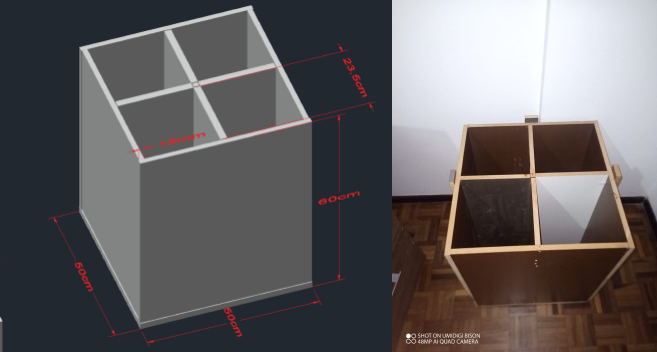
\includegraphics[width=10cm]{Figures/Container Block.png}
  \caption{\small{Container section model}}
  \label{fig:containerModel}
\end{figure}

The second modeled part was the sorting section. Following the container section constraints, the sorting part has 50x50cm dimension and 40cm height. It houses two of the three flaps and motors as well as four ultrasonic sensors. To protect the components and wires connecting to the micro-controller a hollow middle section was designed, containing only hole near one of the walls to allow wires to be passed through.

\begin{figure}[H]
  \centering
  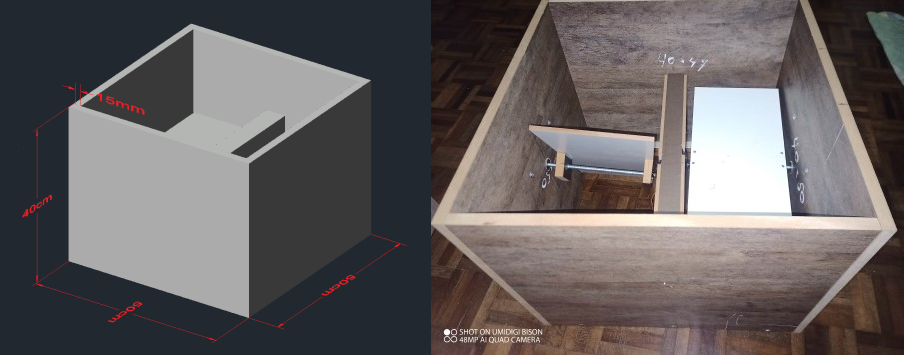
\includegraphics[width=10cm]{Figures/Sorting1.png}
  \caption{\small{Sorting section model}}
  \label{fig:sortingModel1}
\end{figure}

As mentioned before, the flaps are sustained by a 8mm iron bar attached to a ball bearing in the opposite side of the motor. This allow the motor to freely rotate while providing good resistance to weights falling in the flaps.

\begin{figure}[H]
  \centering
  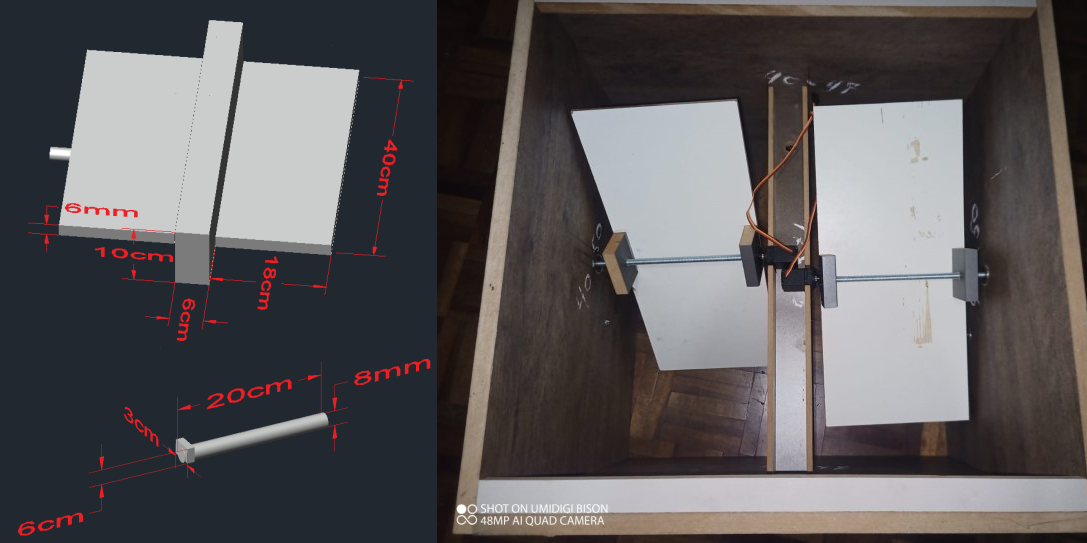
\includegraphics[width=10cm]{Figures/Sorting2.png}
  \caption{\small{Sorting flaps iron axis}}
  \label{fig:sortingModel2}
\end{figure}

Lastly the cover section was modeled. It was designed in a way that separates the electronic components from the waste that would be thrown inside the Smart Recycler.

\begin{figure}[H]
  \centering
  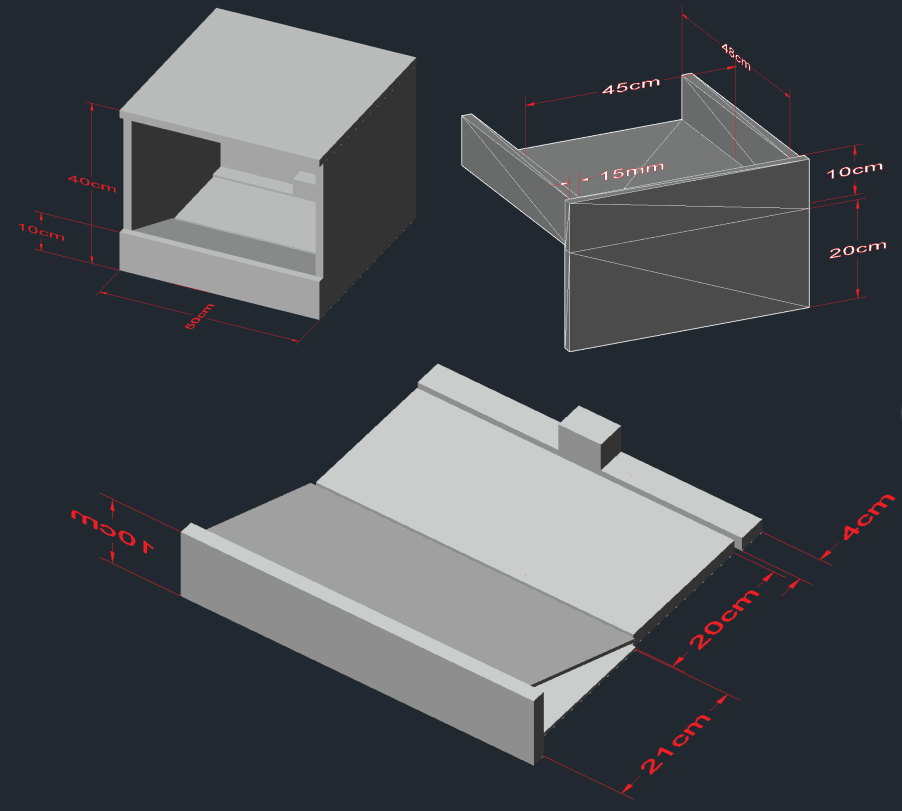
\includegraphics[width=10cm]{Figures/Cover Model.png}
  \caption{\small{Cover section model}}
  \label{fig:coverModel1}
\end{figure}

\begin{figure}[H]
  \centering
  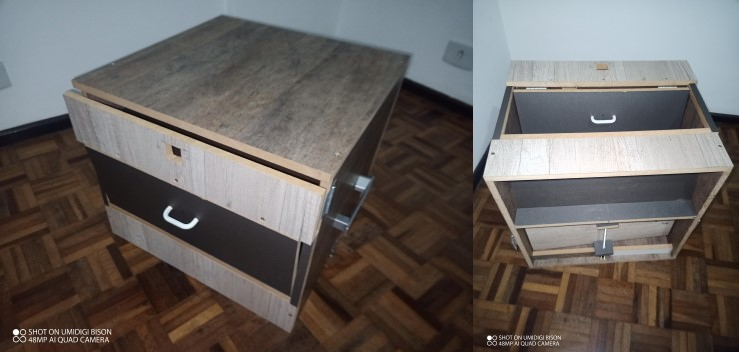
\includegraphics[width=10cm]{Figures/Cover Built.png}
  \caption{\small{Cover section built}}
  \label{fig:coverModel2}
\end{figure}

The final assembled structure can be seen in the following figure:

\begin{figure}[H]
  \centering
  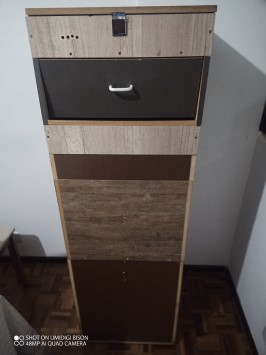
\includegraphics[scale=0.7]{Figures/Full Structure.jpg}
  \caption{\small{Assembled mechanical structure}}
  \label{fig:fullBody}
\end{figure}

\subsection{Hardware Components}
\subsubsection{Module Esp32-Cam Ov2640 2MP}
The ESP32-CAM is a small size, low-power consumption camera module based on ESP32. It comes with an OV2640 camera and provides an onboard TF card slot \cite{evelta}.

\begin{figure}[H]
  \centering
  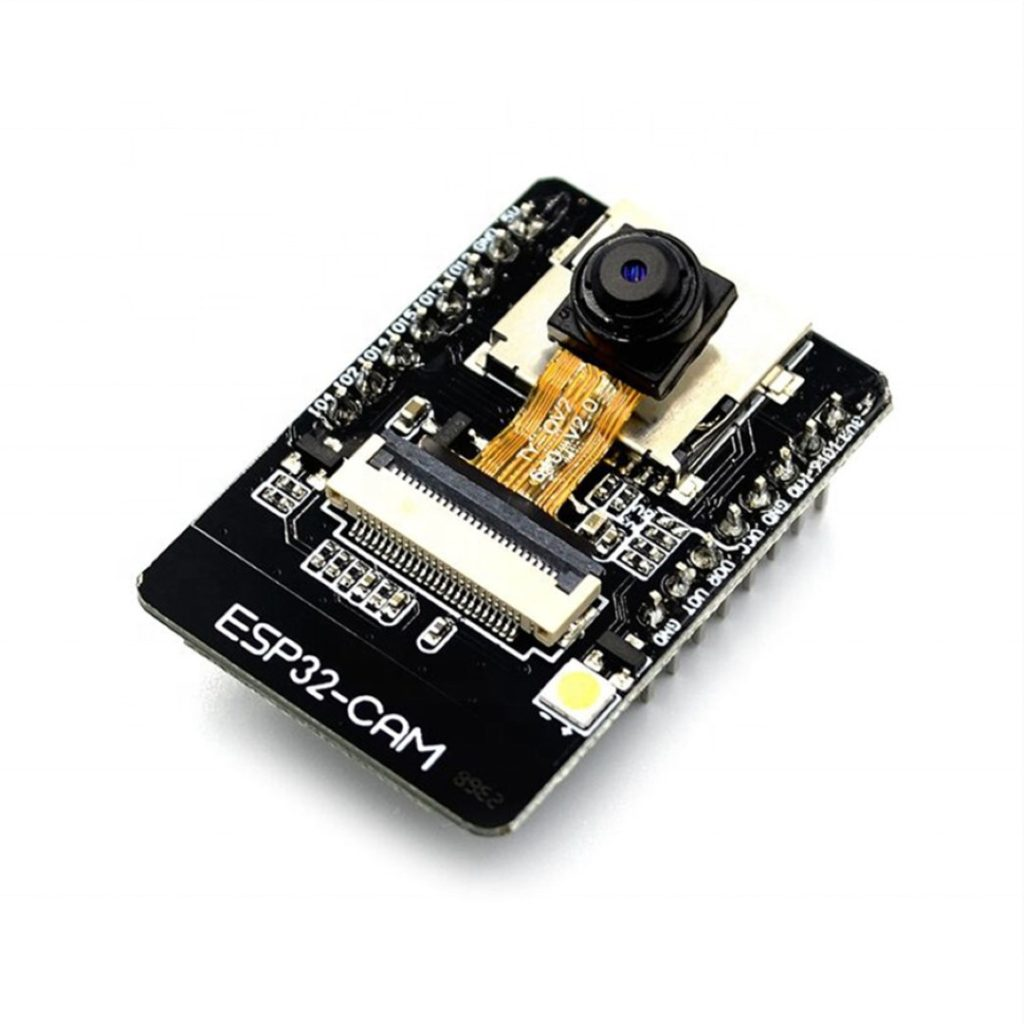
\includegraphics[width=5cm]{Figures/esp32cam-1024x1024.jpg}
  \caption{\small{Esp32-Cam Module}}
  \label{fig:Esp32}
\end{figure}

With a wide range of uses, from wireless video monitoring to QR identification, the Esp32 was chosen for this project due to its WiFi image upload capacity. But due to its low number of GPIO ports, it was necessary the utilization of another processing unit.

\subsubsection{Arduino Mega 2560 R3}
The Arduino Mega 2560 is a micro-controller board based on the ATmega2560. The selection of this micro-controller board as one of the main processing units of this project took into account the number of digital input/output pins, the supported number of PWM outputs, low cost, familiarity, and ease of use of the component by the members of the team\cite{arduino}.In this project, the mega is responsible for controlling most of the system, such as the rotation of the flaps, verification of ultrasonic and infrared sensors, activation of the led tape, communication with ESP32, and the displayed messages in the OLED display. it also has an easy-to-use interface with most of the peripherals.

\begin{figure}[H]
  \centering
  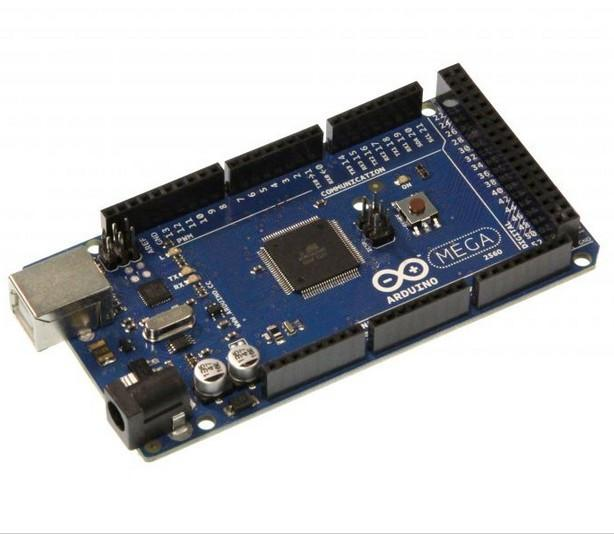
\includegraphics[width=5cm]{Figures/arduinoMega.jpg}
  \caption{\small{Arduino Mega 2560}}
  \label{fig:Arduino}
\end{figure}

\subsubsection{Lead-Acid Battery Zebra Ps4024}
To make the project more portable, we decided to use a battery as a power supply. So it was chosen a rechargeable Lead-Acid Battery with a 12V-7Ah output, capable to supply the whole system for over 48 hours.

\begin{figure}[H]
  \centering
  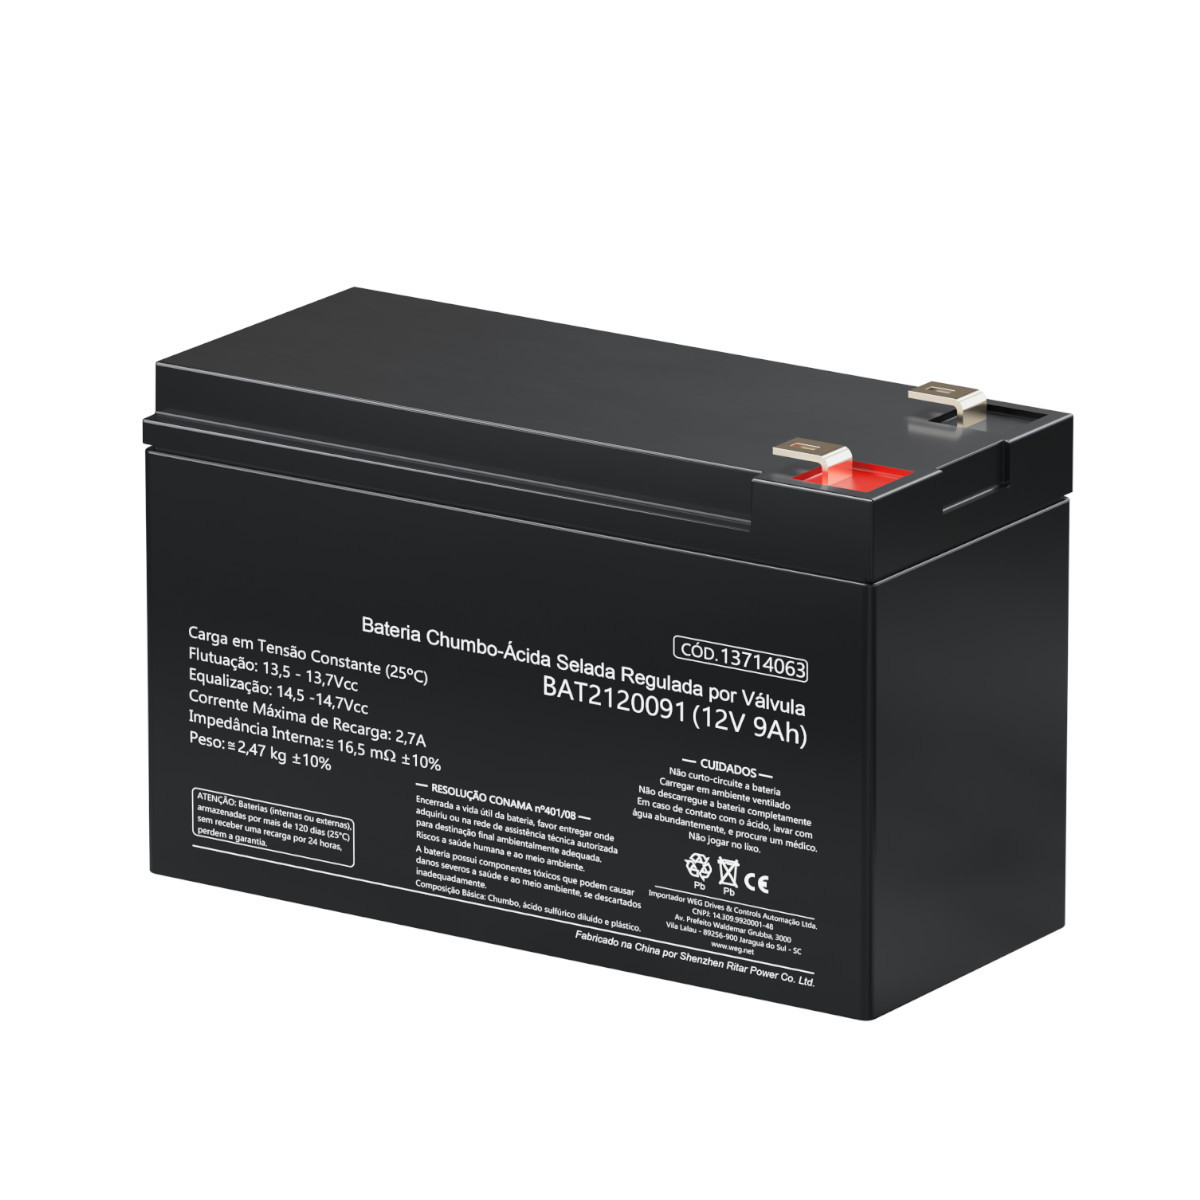
\includegraphics[width=5cm]{Figures/WDC_Bateria_VRLA_9AH_12V_1200Wx1200H.jpg}
  \caption{\small{Lead-Acid Battery}}
  \label{fig:Battery}
\end{figure}

\subsubsection{Voltage regulator lm2596}
Due to its voltage output of 12V, it was necessary a step-down regulator to safely supply the peripherals. There are three regulators, one for the servo-motors with an output of 6V, one for the Arduino mega with an output of 9V, and a third one for the other components with an output of 5V. To avoid noise, the grounds of the regulator of the servo-motors and the rest of the system are joined by a single point.

\begin{figure}[H]
  \centering
  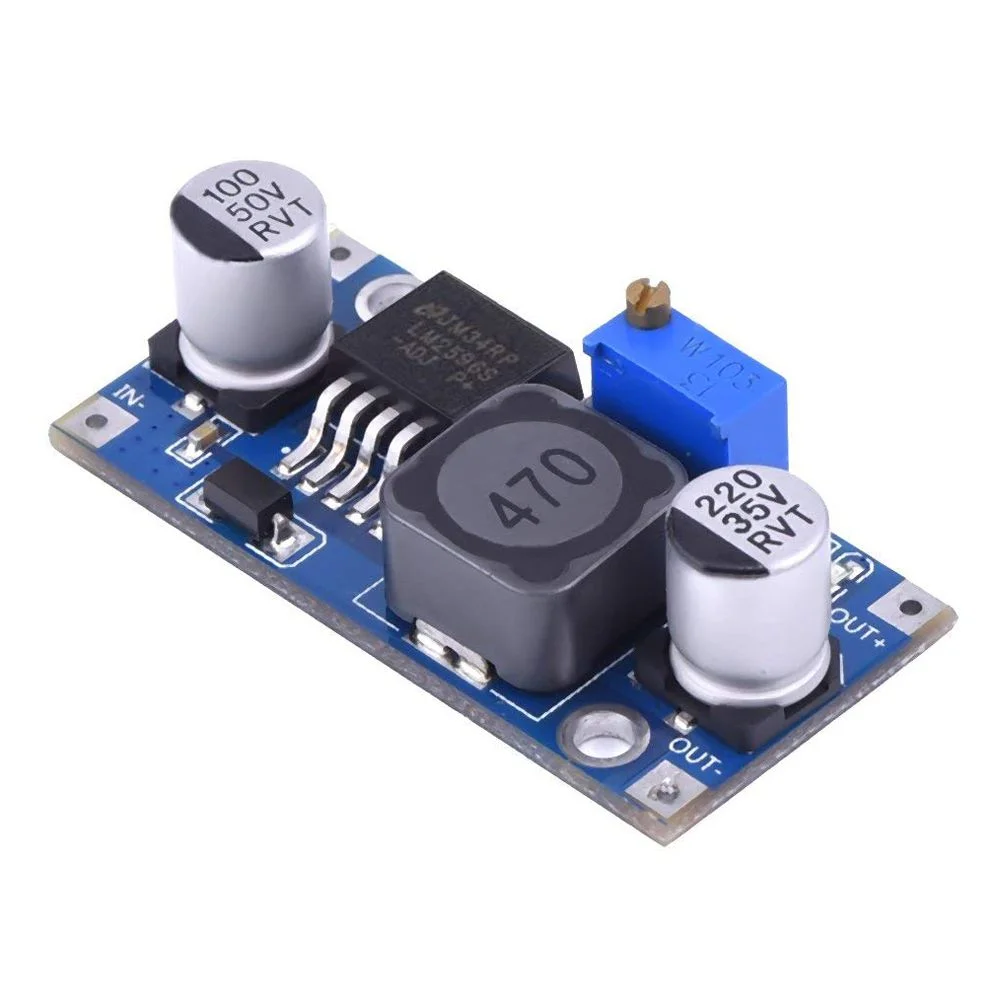
\includegraphics[width=5cm]{Figures/voltageRegulator.jpg}
  \caption{\small{Voltage regulator Step-down LM25960}}
  \label{fig:VoltageRegulator}
\end{figure}

\subsubsection{High Torque Servo Motor Mg996r}
This High-Torque MG996R Digital Servo features metal gearing resulting in extra high 10kg stalling torque per cm in a tiny package. This high-torque standard servo can rotate approximately 180 degrees (90 in each direction). \cite{servo}

\begin{figure}[H]
  \centering
  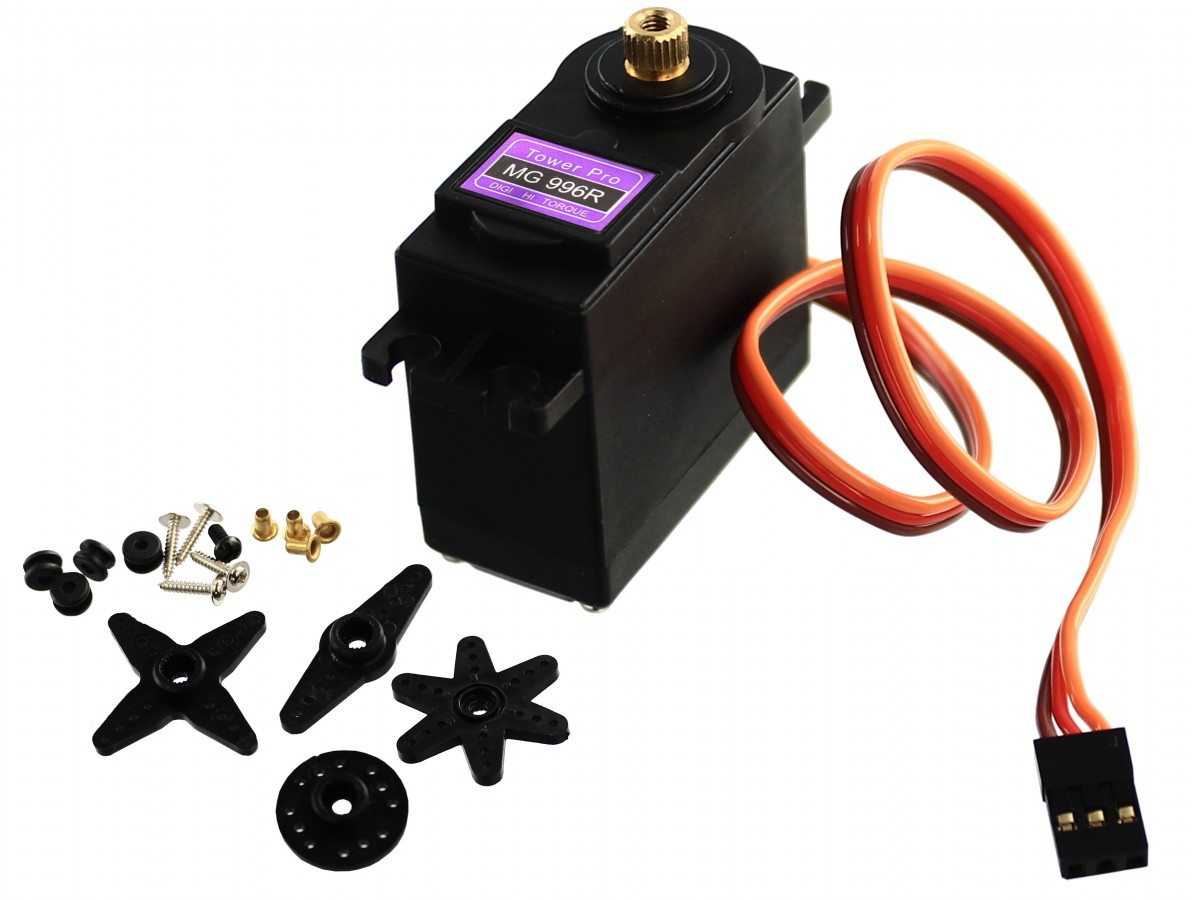
\includegraphics[width=5cm]{Figures/servo-motor-mg996r-tower-pro-360-11kgcm-rotacao-continua-com-engrenagens-metalicas.jpg}
  \caption{\small{Servo motor mg996r}}
  \label{fig:servo}
\end{figure}

In this project were used three of such servos to do a precise flap control, with them being controlled by the Arduino mega. To take into account the noise generated by the servos it was also put a 47 $\mu$F capacitor between the 6V and ground.

\subsubsection{Infrared Sensor Ir Lm393}
This simple to use infrared sensor, being supplied 5V with an output pin to indicate the present state, was used in the system to detect the opening of the gate, which was used to reference the input of items in the bin.

\begin{figure}[H]
  \centering
  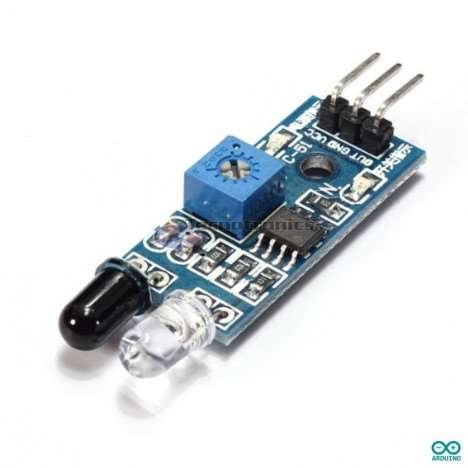
\includegraphics[width=5cm]{Figures/infraRed_sensor.jpg}
  \caption{\small{Infra Red Sensor}}
  \label{fig:ir}
\end{figure}

\subsubsection{OLED Display 1.6" \space LCD}
As one of the interfaces with the user, this display shows to them several messages and the QR code that will be used to redeem the credits in the web app. This display has a 130x130 resolution and an I2C interface. It permits the the creation of graphs, in our case QR codes, and texts with ease.

\begin{figure}[H]
  \centering
  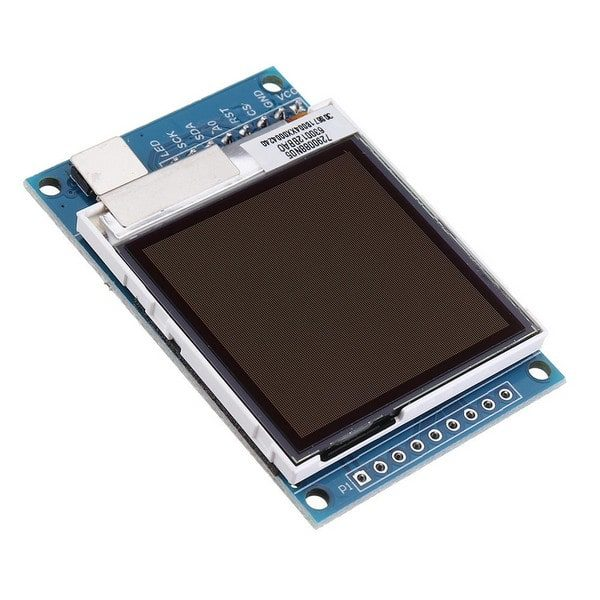
\includegraphics[width=5cm]{Figures/Display-LCD-TFT-1.6-130x130-Transflectivo-6-600x600.jpg}
  \caption{\small{OLED Display 1.6 inches}}
  \label{fig:display}
\end{figure}

\subsubsection{Ultrasonic Sensor Hc-sr04}
HC-SR04 is an ultrasonic ranging module that provides 2 cm to 400 cm non-contact measurement function\cite{ultrasonic}. This module is used as a means to discover when the compartment bins got full by getting the distance between them and the closest trash.

\begin{figure}[H]
  \centering
  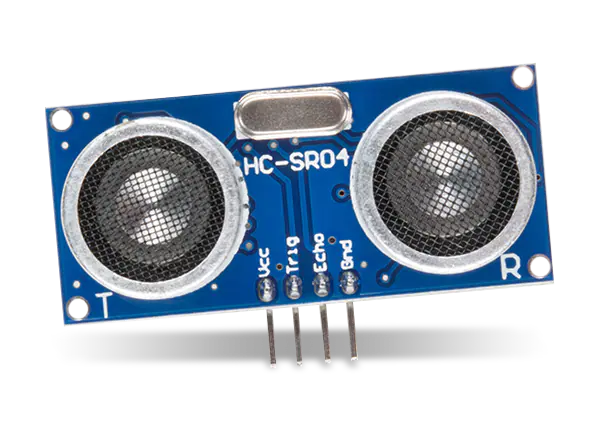
\includegraphics[width=5cm]{Figures/ultrasonico_hc.jpg}
  \caption{\small{Ultrasonic Sensor hc-sr04}}
  \label{fig:ultrasonic}
\end{figure}

\subsubsection{Led Tape 3528 White}
In this project, good quality pictures of the items disposed is a vital requirement, so it was necessary to create a well illuminated environment inside the chamber. To solve this problem it was used a 12V led tape that, in the closed chamber, provided a constant and clear light source.

\begin{figure}[H]
  \centering
  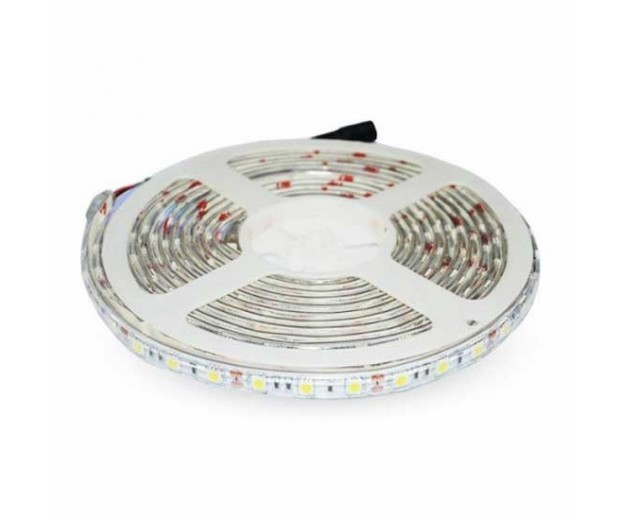
\includegraphics[width=5cm]{Figures/ledtape.jpg}
  \caption{\small{Led Tape}}
  \label{fig:ledtape}
\end{figure}

\subsubsection{Red LED's}
With the necessity to indicate the fact that one or more of the containers are full, it was implemented in this project one red led for each bin. This way if the red led of a respective bin is on, then the respective container is full and needs to be depleted.

\subsection{Electronic Circuit}
Beginning the project with the testing of all the components individually, making sure of their use and functionality, it was then necessary the creation of the first design of the electronic circuit. After the test of this first design on a breadboard, it was noticed some noises that were affecting the system. So to resolve this issue three capacitors were added, two between the 5V and ground and one between 6V and ground. Finally everything was assembled on the standard board.

The ESP32-Cam is powered by the 5V regulator and communicates with the Arduino board via UART. The servo-motors that control the flaps, powered by the 6V regulator, are connected to the PWM pins of the Arduino board. The infrared, used to detect the opening of gate, is powered by the 5V regulator and directly connected to the Arduino's GPIO. The led tape is directly connected to the 12V battery and a relay module. The relay module is then connected to the 5V regulator and the GPIO pin of the Arduino. The ultrasonic sensors are powered by the 5V regulator with the trigger pin connected to the GPIO and the echo pin to the PWM pins in the Arduino. The OLED display is powered by the 5V regulator and communicates with the Arduino via the I2C pins.

As shown in the figure \ref{fig:circuit}, bellow.

\begin{figure}[H]
  \centering
  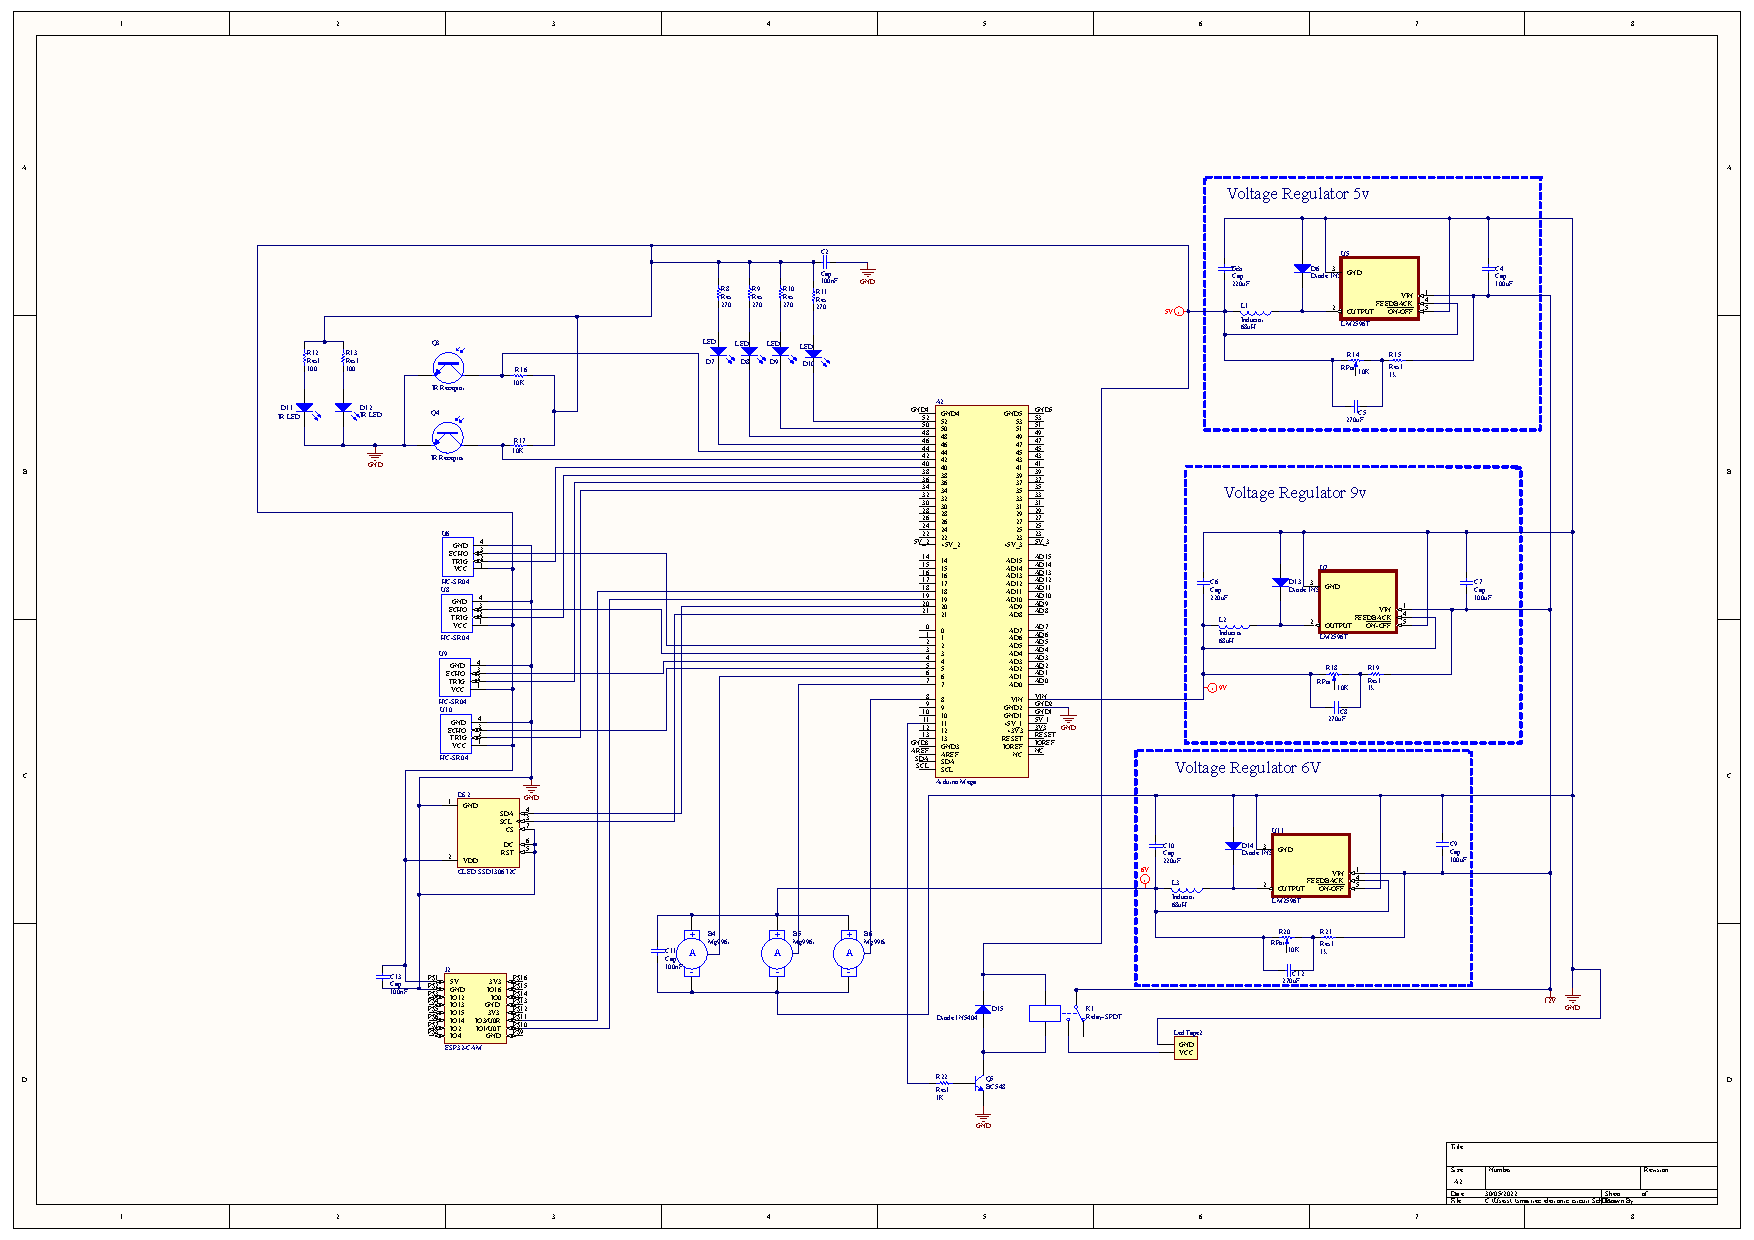
\includegraphics[width=17.8cm, angle=-90]{Figures/Eletronical Circuit.pdf}
  \caption{\small{Electronic circuit made with Altium}}
  \label{fig:circuit}
\end{figure}

\subsection{Firmware}
Since the project consists of two micro-controllers two firmware's were created, one for the ESP32 and other for the Arduino Mega. The ESP32-Cam firmware was the first to be coded and, as pointed before, its purpose is to take pictures of the waste items inside the Smart Recycler and communicate with the back end. Initially the micro-controller keep trying to establish a connection with a specified WiFi network only proceeding when successful.

Once connected, the micro-controller awaits an OK signal from the Arduino Mega through its UART port. When this signal is received a timeout period of 10 seconds is started, activating the embedded camera. While the timeout period has not expired the micro-controller will then attempt to take a picture of the item inside.

With the image captured the ESP32-Cam then tries to establish a connection with the back end so the image can be send using \textit{HTTP POST} protocols. The received response from the back end is a \textit{JSON} string that is parsed using the \textit{ArduinoJSON} library \cite{ArduinoJson}. Finally, a response is sent to the Arduino Mega in a \textit{JSON} format containing the host IP address, image classification and redeem code that will be used by the Arduino Mega to generate a \textit{QR Code} to be displayed to the user.

The final ESP32-Cam firmware behavior can be seen in the state diagram in the following figure:

\begin{figure}[H]
  \centering
  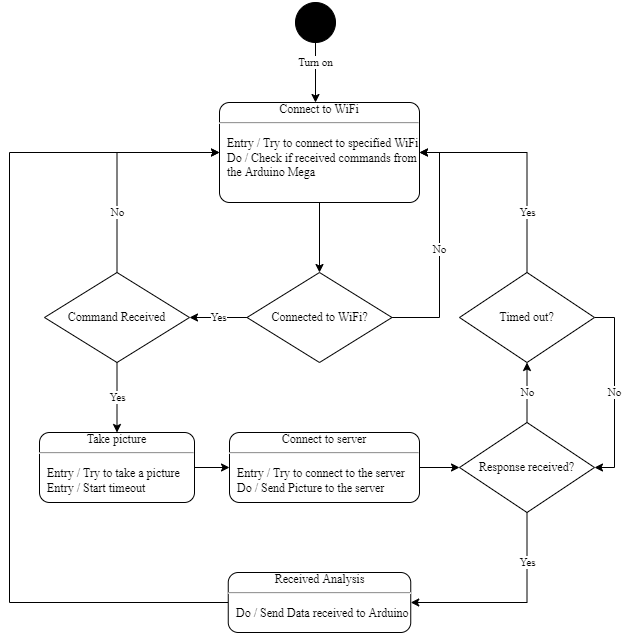
\includegraphics[width=12cm]{Figures/State Chart Esp32.png}
  \caption{\small{Esp32-Cam state diagram}}
  \label{fig:espState}
\end{figure}

The Arduino Mega is the second micro-controller and is the main responsible for handling the components in the project. Initially it keeps reading the infrared sensor until something is detected, starting the recycle process. Once this process begins, the Arduino Mega sends through the UART connection with the ESP32-Cam an OK message and a 15 seconds timeout is started. If no expected message from the ESP32-Cam is received during this period, the item inside will be recycled to the \textit{Other} container by default.

After receiving a response from ESP module the Arduino will then generate and display a \textit{QR Code} in the oled display for the user and based on the classification received the motors will be rotated accordingly. It is worth to note that the motor from the first level must fully complete its movement before any of the motors from the second level begin theirs, so they won't collide with each other.

After properly disposing of the item, the four ultrasonic sensor are measured, updating the fill level of each container. If any of the containers are filled enough so that the amount of waste inside it is within 10cm of the ultrasonic sensor the respective led will be turned on, signalizing that such container is full and no more waste can be disposed there. If a container is full and an item that should be disposed in such container is thrown inside the recycler, it will be directed to the \textit{Other} container instead.

The final Arduino Mega firmware behavior can be seen in the state diagram in the following figure:

\begin{figure}[H]
  \centering
  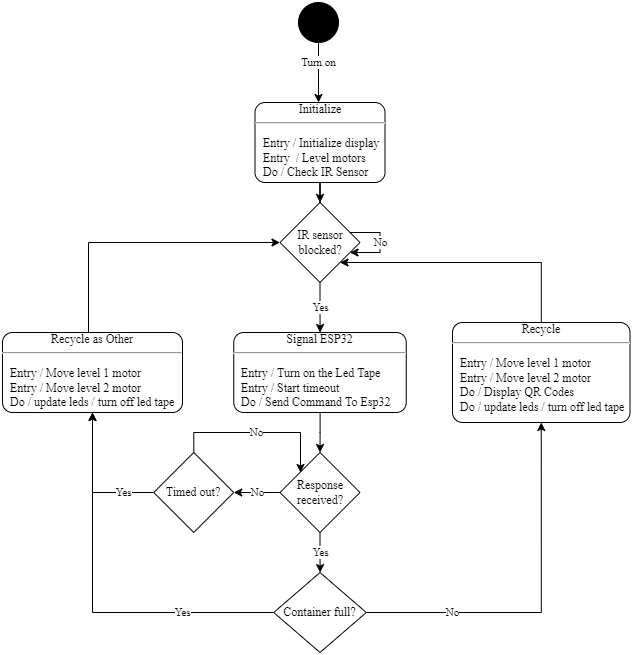
\includegraphics[width=12cm]{Figures/State chart Arduino Mega.png}
  \caption{\small{Arduino Mega state diagram}}
  \label{fig:arduinoState}
\end{figure}

\subsection{Back end}
With the Flask framework, three different types of routes were created to expose the application functionalities, they were user related routes, transaction related routes, and classification related routes.
There are three routes related to users, one GET to acquire user information and two POSTs to sign in and sign up the user. User information is stored in the users database, and its password information is stored encrypted so that only the user knows its own password.
There are two routes related to transactions, one POST to send transactions between users and other POST to give the user credits when redeeming a redeem code. Transactions require the username of the sender and the receiver and the amount to send, checks are made to ensure only proper transactions happen.
Finally, there’s two routes related to classifications, one POST that receives an image and returns the classification that the neural network model loaded thinks is most likely to be in the image and one GET route to get statistics about all the classifications made.
In the Figure \ref{fig:backend_route} is an example of request and response from the Back end.

\begin{figure}[H]
  \centering
  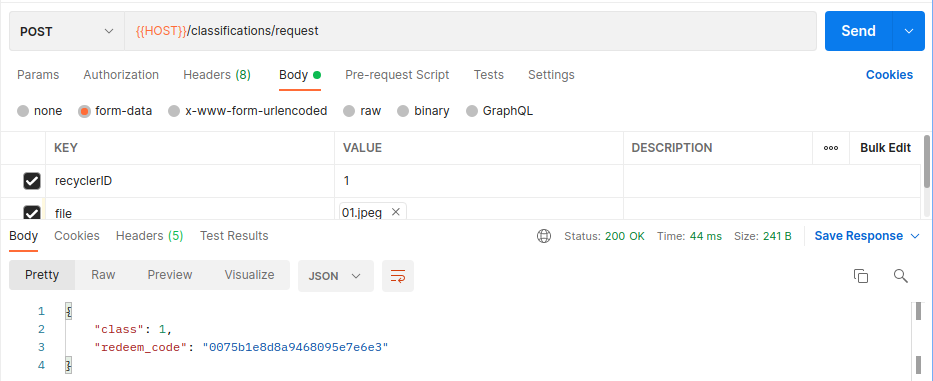
\includegraphics[width=12.5cm]{Figures/backend_classification_request.png}
  \caption{\small{Backend route example}}
  \label{fig:backend_route}
\end{figure}

\subsection{Web Application}
The web application was created so the user has an easy and functional way of interacting with the Smart Recycler, a web application was made instead of a native mobile application since it would be much easier for users to redeem credits if they don’t need to download a mobile application.
The web application is divided into two states: non-authenticated and authenticated. When non-authenticated, the user can sign in and sign up using the corresponding pages. When authenticated, the user can redeem credits, check its account balance, send credits to other users, and check Smart Recycler statistics. The redeem credits functionality works by the user reading the URL contained in the QR code sent by the Smart Recycler and being redirected to the web application, which will store redeem code information using browser cookies if the user is not authenticated and send the redeem credits to the Back end if the user is authenticated. Finally, to send credits the user only needs to specify the receiver and the amount to send.
In the Figure \ref{fig:front_pages} all web application pages are shown.

\begin{figure}[H]
  \centering
  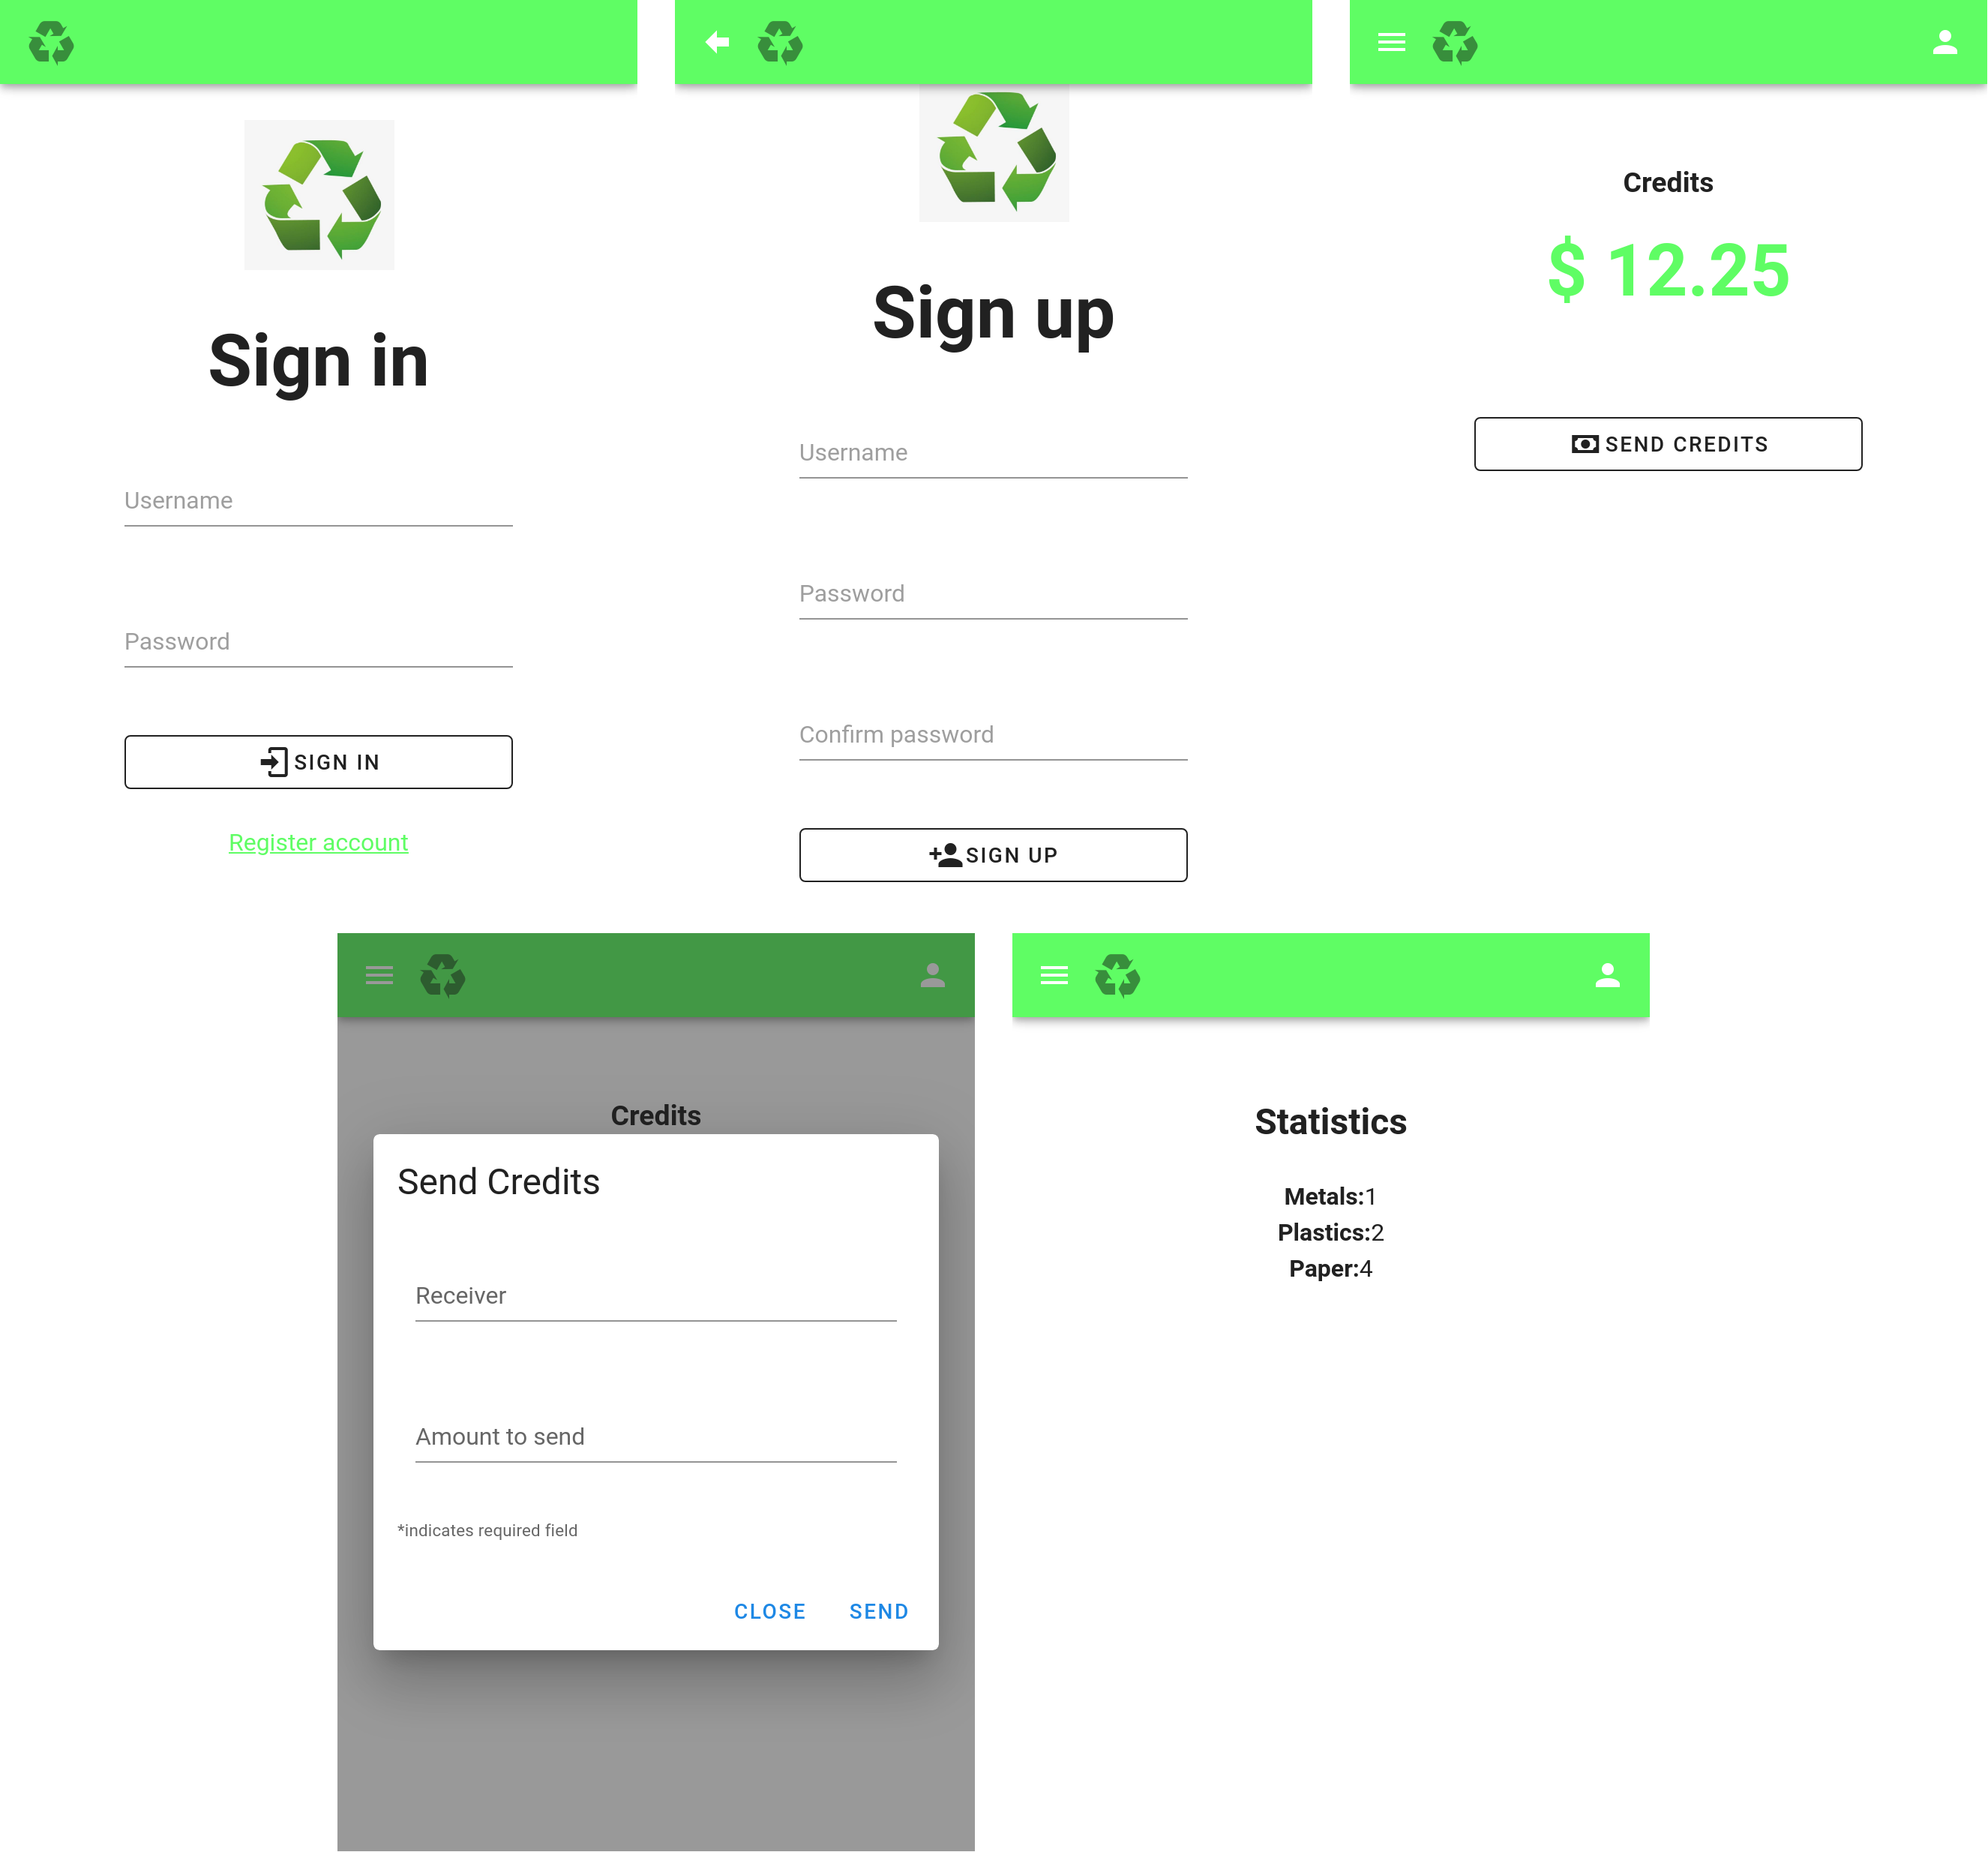
\includegraphics[scale=0.1]{Figures/front_pages.png}
  \caption{\small{Web Application pages}}
  \label{fig:front_pages}
\end{figure}

\subsection{Inference System}
The inference system was one of the hardest parts to develop in the project, since we had a problem specific to our project, which was detecting some types of trash thrown in the Smart Recycler, a custom dataset was needed to properly classify our desired objects. To create this custom dataset, we used an embedded software that was uploaded in the ESP32 to take images and upload them in a Google Drive folder, allowing us the fast creation of a dataset with images taken directly from inside the Smart Recycler top compartment. Then we used an object tagging tool, VoTT, to annotate the images with the desired classes that we wanted to classify, in the Figure \ref{fig:annotation_example} is an example of the annotation process.

\begin{figure}[H]
  \centering
  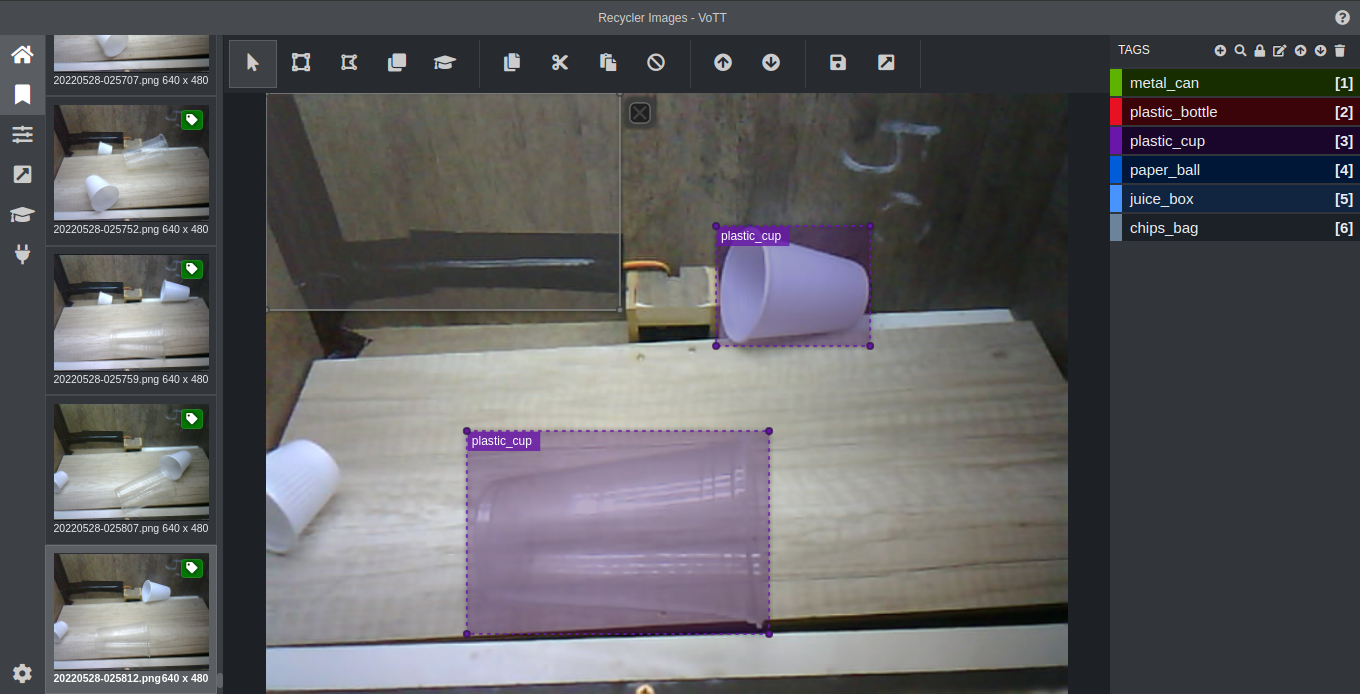
\includegraphics[width=12.5cm]{Figures/annotation_example.png}
  \caption{\small{Annotation examples}}
  \label{fig:annotation_example}
\end{figure}

After annotating and dividing the images in the desired classes, we split the dataset into training, validation, and testing dataset in a ratio of roughly 70\%, 10\%, and 20\% respectively. The training dataset is used by the neural network API to improve its inference accuracy, the testing dataset is used in the training phase to check the model metrics and the validation dataset is used later to test the model with images outside of the training process. To increase the model’s ability to detect different situations, we augment the training and testing dataset, where each image generates six other images with certain possible transformations. The augmentations used were the following: gaussian blur with 50\% chance, salt and pepper noise with 25\% chance, gamma contrast chan\-ge with 25\% chance, and affine transformations as scaling and rotating the images. In the Figure \ref{fig:augmentation_example}, an example of the augmentation is shown.

\begin{figure}[H]
  \centering
  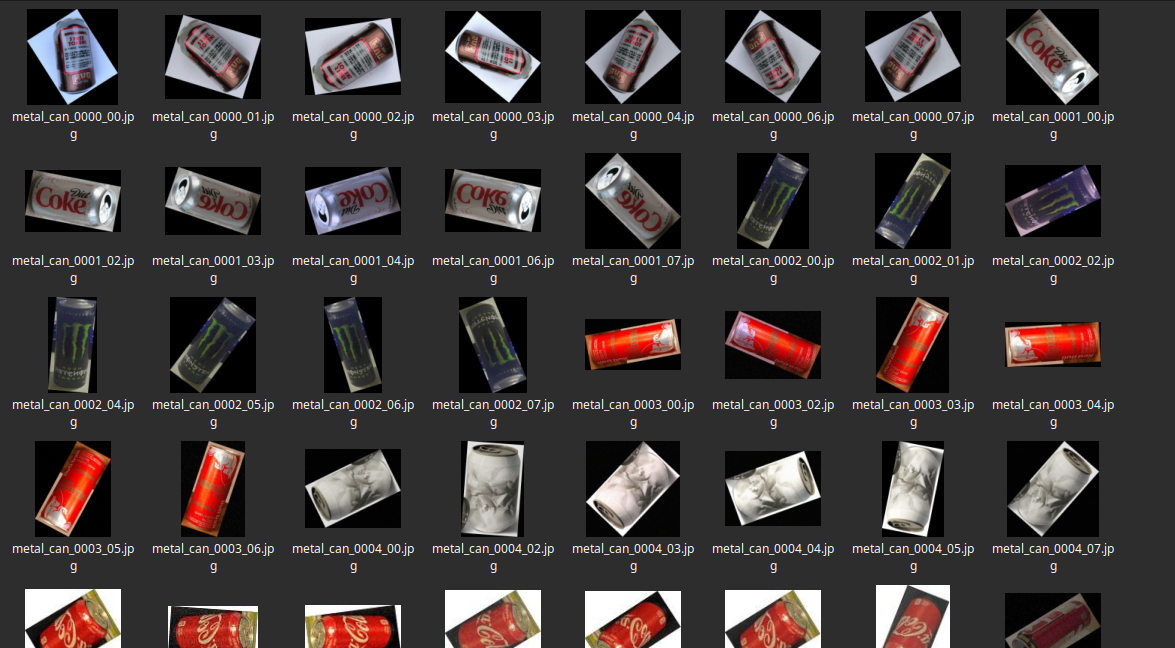
\includegraphics[scale=0.3]{Figures/Training directory example.png}
  \caption{\small{Augmentation output}}
  \label{fig:augmentation_example}
\end{figure}

For the training process, multiple parameters must be chosen, the technique used to speed up network training was the transfer learning, where pre-trained weights are used so only the top layers of the network need to be trained again, using pre existing feature detectors from the last layers, the ImageNet weights were used to transfer learn from. There are multiple possible networks that can be chosen to create our model, some of the trained networks were: ResNet50V2, MobileNet, InceptionV3, and EfficientNet. The chosen network was the EfficientNetB4 for its moderate size and high accuracy in our dataset. The activation function used was the sigmoid function, since it’s an activation function that allows multiple class inferences to be made by each model prediction. After each epoch in the training process, the network is evaluated and accuracy is calculated, if accuracy increases, the model is saved in the file system. The Figure \ref{fig:training_model} showcases the plotting of the evolution in the loss and accuracy metrics in the training and validation datasets.

\begin{figure}[H]
  \centering
  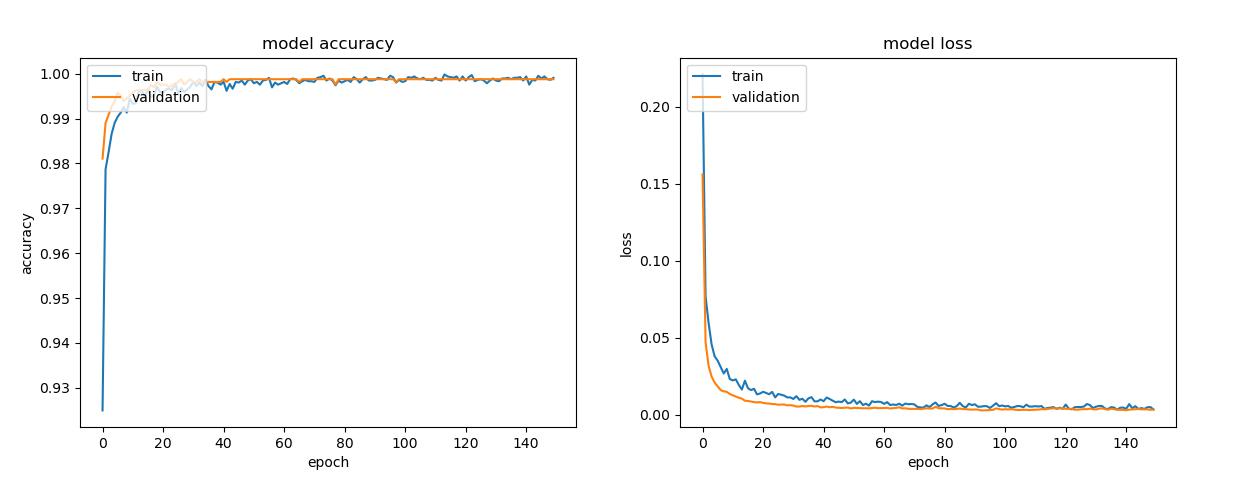
\includegraphics[width=12.5cm]{Figures/training_result.png}
  \caption{\small{Accuracy and Loss graphs from the trained model}}
  \label{fig:training_model}
\end{figure}

\subsection{Budget}
The following table details the project budget and the amount of money spent on every item. The total estimated cost of the project was R\$ 838,00 but during the development the ESP32-Cam micro-controller was damaged and had to be replaced, increasing the final budget by R\$ 86,00, totaling R\$ 924,00 which was divided between three team members or R\$ 308,00 each.

% Budget table
\begin{table}[H]
  \small
  \caption{\small{Budget}}
  \begin{center}
    \begin{tabular}{|l|c|l|l|}
      \hline
      \textbf{Item}                           & \textbf{Qnt} & \textbf{Unit Cost} & \textbf{Total Cost} \\ \hline
      Arduino Mega 2560 R3                    & 1            & R\$ 114,00         & R\$ 114,00          \\ \hline
      Voltage Regulator Xl4015                & 1            & R\$ 44,00          & R\$ 44,00           \\ \hline
      Lead-Acid Battery Zebra Ps4024          & 1            & R\$ 130,00         & R\$ 130,00          \\ \hline
      High Torque Servo Motor Mg996           & 4            & R\$ 50,00          & R\$ 200,00          \\ \hline
      Infrared Sensor Ir Lm393                & 1            & R\$ 12,00          & R\$ 12,00           \\ \hline
      Oled Display 1.6 LCD Pic 130*130        & 1            & R\$ 60,00          & R\$ 60,00           \\ \hline
      Module Esp32-Cam Ov2640                 & 2            & R\$ 86,00          & R\$ 172,00          \\ \hline
      Ultrasonic Sensor Hc-sr04               & 4            & R\$ 15,00          & R\$ 60,00           \\ \hline
      Led Tape 3528 White                     & 1            & R\$ 32,00          & R\$ 32,00           \\ \hline
      Other materials/components/replacements & 1            & R\$ 100,00         & R\$ 100,00          \\ \hline
      \textbf{Total}                          & -            & -                  & \textbf{R\$ 924,00} \\ \hline
    \end{tabular}
  \end{center}
  \label{tab:budget}
\end{table}

\subsection{Schedule}
The table below details the estimated and worked hours during the development of the project over the course of nine weeks.

% Schedule table
\begin{table}[H]
  \small
  \caption{\small{Schedule}}
  \begin{center}
    \begin{tabular}{|l|l|l|}
      \hline
      \textbf{Deliverable}           & \textbf{Estimated Hours} & \textbf{Worked Hours} \\ \hline
      Blog Page and Project Planning & 52                       & 46                    \\ \hline
      Mechanical Project             & 33,5                     & 34,5                  \\ \hline
      Hardware Project               & 43                       & 46,8                  \\ \hline
      Software Project               & 70,5                     & 74,5                  \\ \hline
      Integration                    & 50                       & 48                    \\ \hline
      Overall Integration and Tests  & 42                       & 51                    \\ \hline
      Documentation                  & 18                       & 25,5                  \\ \hline
      Blog Keeping and Meetings      & 31                       & 31                    \\ \hline
      \textbf{Total}                 & \textbf{340}             & \textbf{357,3}        \\ \hline
    \end{tabular}
  \end{center}
  \label{tab:schedule}
\end{table}

\section{Results}
Despite being a mechanically complex project, with several challenges such as movement coordination and image classification, some good results were obtained in the end and the team believes that such a system could be beneficial if implemented in any environment, not only in the planned one. Some major problems presented themselves along the development, such as the low accuracy of the first trained inference system and the handling of the motors when dealing with heavy objects.

The first trained neural network was based on the \textit{ResNet50V2} and despite presenting a accuracy of 86,47\% in the training, which was within the required range of 80\%, when put to test in a real scenario it performed poorly for a couple of classes as can be seen in the figure \ref{fig:resnet}

\begin{figure}[H]
  \centering
  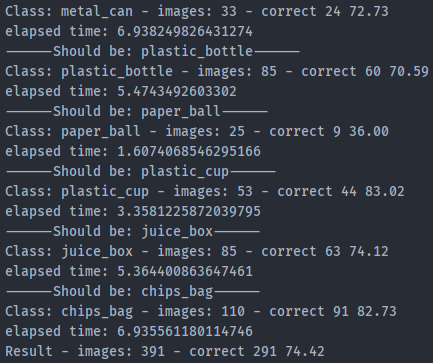
\includegraphics[width=10cm]{Figures/ResNet50V2-E150-6C-0-PRED.png}
  \caption{\small{ResNet50V2 inference prediction}}
  \label{fig:resnet}
\end{figure}

The resultant network was also quite heavy with over 90 MB in size and with a model loss that almost reached 40\%.

\begin{figure}[H]
  \centering
  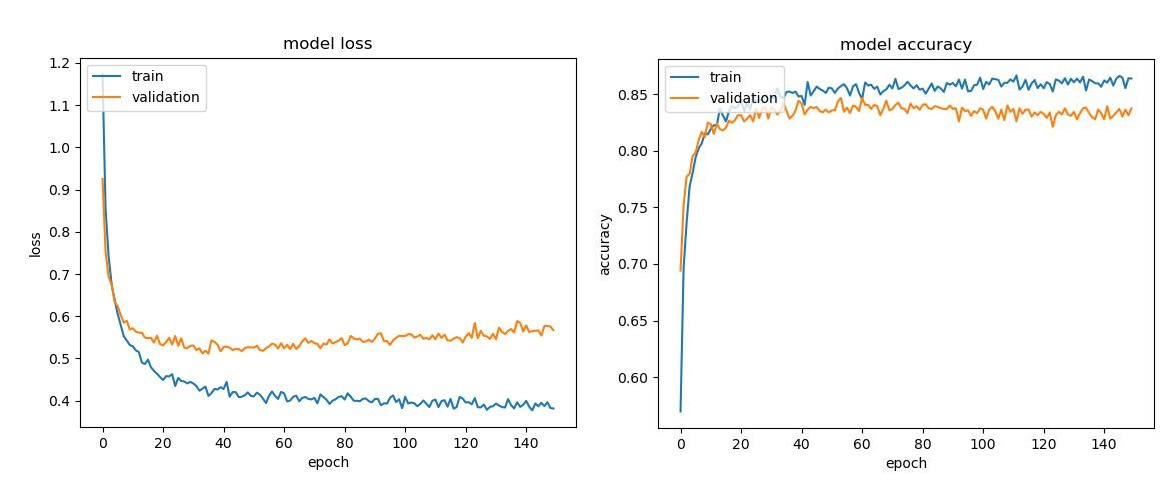
\includegraphics[width=12cm]{Figures/ResNet50V2_Loss_Acc.jpg}
  \caption{\small{ResNet50V2 loss and accuracy}}
  \label{fig:resnetLossAcc}
\end{figure}

The second network trained was based on the \textit{MobileNetV2} model and the team was expecting good results from this network because of its size. In comparison with the other trained models, this one is very small, with approximately 9 MB in size and despite presenting a similar accuracy and loss as the \textit{ResNetV2} with 86,71\% accuracy and 37,28\%, when put to the test in a real scenario it performed a little worst.

\begin{figure}[H]
  \centering
  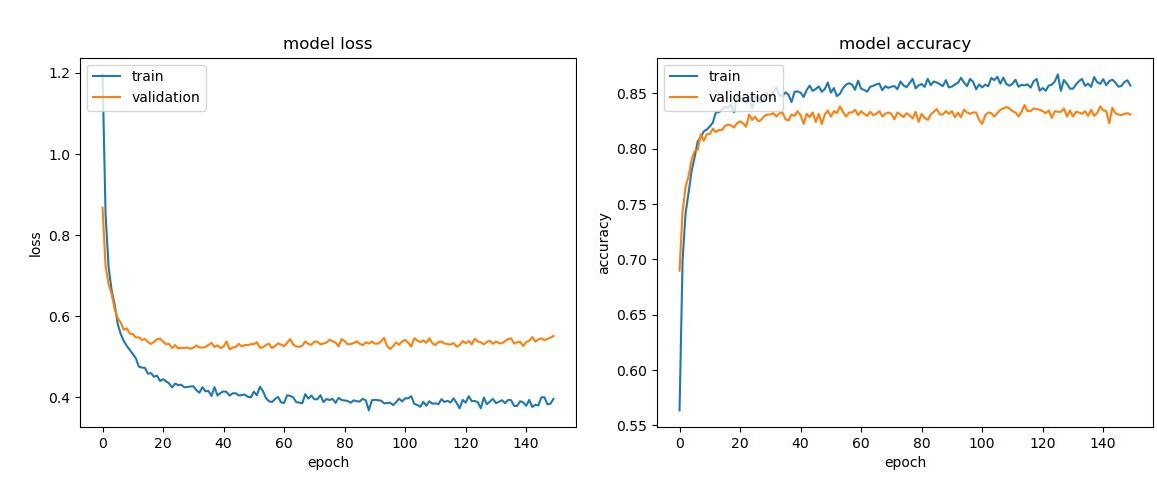
\includegraphics[width=12cm]{Figures/MobileNetV2_Loss_Acc.jpg}
  \caption{\small{MobileNetV2 loss and accuracy}}
  \label{fig:mobilenet}
\end{figure}

Thankfully the \textit{EffecientNetB4} model presented a really good accuracy with 99,98\% and a very low loss with 0,037\% while maintaining a moderate size of approximately 70 MB. The only downside of training this model is the time it takes to finish its training, in our case with 150 epochs taking over 5 hours in a computer with a GTX 1650 TI GPU with 7.5 compute score. Another good result we had is the image quality from inside the cover as can be seen in figure \ref{fig:itens}. This was crucial to the success of the project since it affects the training of the network directly.

\begin{figure}[H]
  \centering
  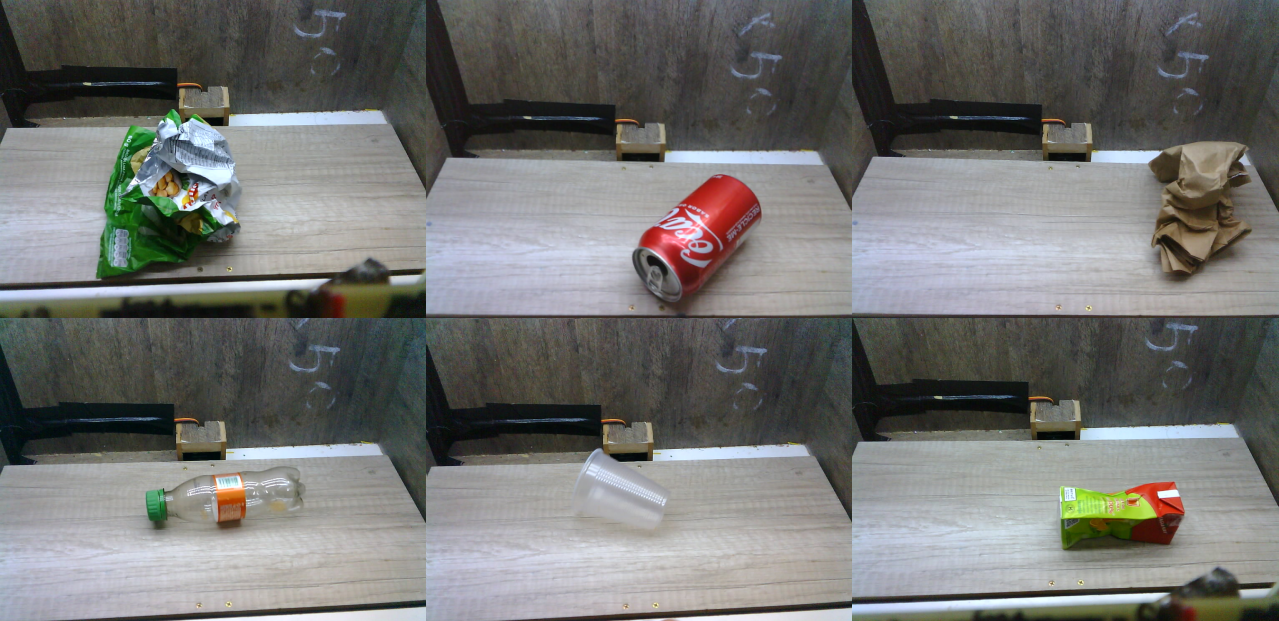
\includegraphics[width=12cm]{Figures/InsideCover.png}
  \caption{\small{Items inside the cover structure}}
  \label{fig:itens}
\end{figure}

% ---------------------------------------------------------------------------- %
%                                 Bibliography                                 %
% ---------------------------------------------------------------------------- %
\bibliographystyle{unsrt}
\bibliography{Bibliography}
\end{document}

